\vspace{3.0ex} \pstart \centering [99 v\textsuperscript{o}] Propositio 1. \pend \vspace{1.0ex} \pstart \edtext{Conatus}{\lemma{perpendiculari.}{\xxref{99vstart}{99vend}}\Afootnote{\textit{ (1) }\ Propositio 1. Conatus simplex\protect\index{Sachverzeichnis}{conatus!simplex|textit} ex medio minus resistente in magis resistens  \textbar\ oblique \textit{ erg.}\ \textbar\ transiens refringitur ad perpendicularem, si contra ex minus resistente in magis resistens  \textbar\ oblique \textit{ erg.}\ \textbar\ intret, refringitur \textit{(a)}\ ad perpendicularem \textit{(b)}\ a perpendiculari. \textit{(aa)}\ Hujus propositionis demonstratio nova non est, repetenda tamen, ut caeteris major Lux\protect\index{Sachverzeichnis}{lux|textit} astet. \textit{(bb)}\ Si \textit{(cc)}\ Sin conatus\protect\index{Sachverzeichnis}{conatus|textit} \textit{ (2) }\ Propositio 1. \textit{(a)}\ Si Conatus simplex\protect\index{Sachverzeichnis}{conatus!simplex|textit} ex medio minus resistente in medium \textit{(aa)}\ transiens \textit{(bb)}\ transit, \textit{(aaa)}\ et \textit{(bbb)}\ linea incidentiae ad superficiem mediorum separatricem \textit{(aaaa)}\ facit angul \textit{(bbbb)}\ angulum obliquum facit \textit{(cccc)}\ refringitur a perpendiculari, si e medio magis resistente in minus resistens transeat refringitur ad perpendicularem. Sed si conatus tr \textit{(b)}\ Conatus simplex \textit{(aa)}\ de \textit{(bb)}\ e [...] rectum \textbar\ refractio nulla est \textit{ erg.}\ \textbar\ , conatusque [...] resistente. Esto \textit{ L}}} 
simplex e medio minus resistente in medium magis resistens oblique transiens refringitur a perpendiculari. Idem e medio magis resistente in minus resistens oblique transiens refringitur ad perpendicularem. Sed si conatus transit perpendiculariter, seu si linea incidentiae ad superficiem mediorum separatricem facit angulum rectum refractio nulla est, conatusque pergit in linea incidentiae continuata, celeritate tamen minore in medio magis resistente, celeritate majore in medio minus resistente.\pend
   %\begin{center}    
   %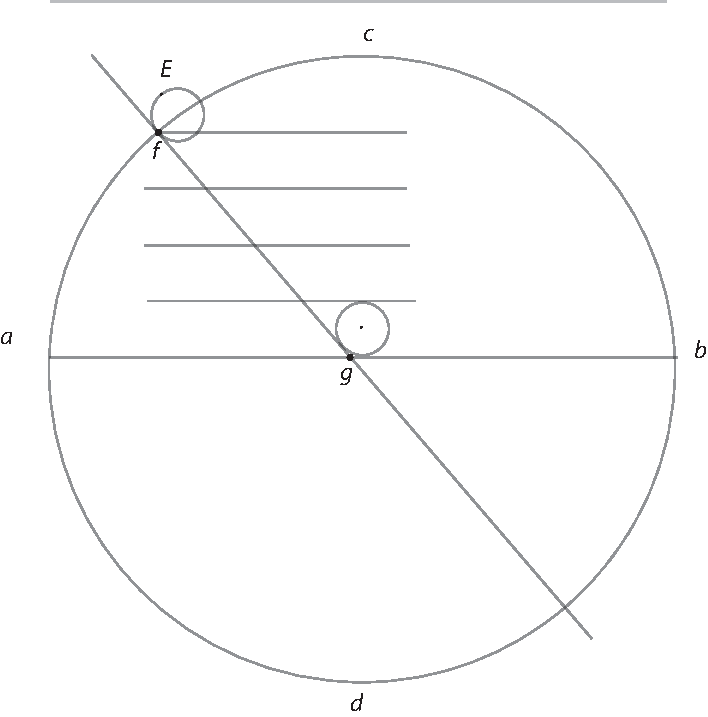
\includegraphics[width=0.7\textwidth]{images/LH37_2_99v_fig1}
   %\\ \vspace{1.0ex} \textit{[Fig. 2, tlw. Blindzeichnung, erster Versuch]}
   %\end{center}
\pstart
   \begin{wrapfigure}{l}{0.5\textwidth}
   \includegraphics[width=0.5\textwidth]
   %Zeitz{images/37_2_99v1}
   {images/LH37_2_99v_fig1}
   \\ \vspace{1.0ex} \centering\textit{[Fig. 2, tlw. Blindzeichnung,\\ erster Versuch]}
   \end{wrapfigure}
Esto\edlabel{99vend} linea separatrix duorum mediorum \textit{ab} corpus \edtext{\textit{E} ponatur ex medio rariore \textit{acb} in densius \textit{adb} transire}{\lemma{corpus}\Afootnote{ \textit{ (1) }\ quod ex medio rariore \textit{acb} \textit{(a)}\ intrat \textit{(b)}\ conatur in densius \textit{adb}, esto \textit{E} punctum ponatur incidere \textit{ (2) }\ \textit{E} [...] \textit{adb} \textit{(a)}\ linea incidere \textit{(b)}\ transire \textit{ L}}} linea incidentiae obliqua \textit{fgh} et si refractio\protect\index{Sachverzeichnis}{refractio} absit continuaturum esse motum in \textit{h}. Patet ante omnia quicquid fertur in linea obliqua \textit{fg} intelligi posse ferri conatibus\protect\index{Sachverzeichnis}{conatus} duobus \edtext{uniformibus}{\lemma{duobus}\Afootnote{ \textit{ (1) }\ aequalibus \textit{ (2) }\ uniformibus \textit{ L}}}, altero in horizontali \textit{fi} ejusque parallelis \textit{lm}, \textit{ng}, aliisque intermediis altero in perpendiculari \textit{fn} ejusque parallelis \textit{op}, \textit{ig} aliisque intermediis, ea celeritatum\protect\index{Sachverzeichnis}{celeritas} inter conatus\protect\index{Sachverzeichnis}{conatus} ratione, quae est linearum cujusque. Nam si corpus \edlabel{estart}\edtext{\textit{E}}{{\xxref{estart}{eend}}\lemma{\textit{E}}\Afootnote{ \textit{ (1) }\ a linea \textit{fn} pergit ire in lineam \textit{op} linea \textit{fi} aut ei aequali et parallela, et eodem tempore ire a linea \textit{fi} in lineam \textit{ng} linea \textit{fn} aut ei aequali et parallela. Patet primum motus punctum fore \textit{f} quod enim simul a linea \textit{fn} et linea \textit{fi} abit necesse est ire ex \textit{f} puncto, solo harum duarum linearum \textit{ (2) }\ intelligatur [...] rectarum \textit{ L}}} intelligatur a linea \textit{fn} ire in rectam \textit{ig} \edtext{[recta]}{\lemma{linea}\Afootnote{\textit{\ L \"{a}ndert Hrsg. } }} \textit{fi} aut ei aequali et parallela, et eodem tempore ire a recta \textit{fi} in rectam \textit{ng} recta \textit{fn} aut ei aequali et parallela. Patet primum motus punctum fore \textit{f} quod enim simul a recta \textit{fn} et recta \textit{fi} abit necesse est ire ex \textit{f} puncto, solo harum duarum rectarum\edlabel{eend} communi. Patet quoque ultimum motus eo tempore absoluti punctum fore \textit{g}. Itur enim simul in rectam \textit{ng} et in rectam \textit{ig}, id est in earum punctum commune \textit{g}.\pend
   \newpage
   \begin{center}
   \includegraphics[width=1.0\textwidth]
%   {images/37_2_99v2}
 {images/LH37_2_99v2}
   \\\textit{[Fig. 3, tlw. Blindzeichnungen]}
   \vspace{1.5ex}
   \end{center}
\pstart Si lineae ex quibus sint \textit{fl} et \textit{fo} lineae ad quas \textit{lp} et \textit{op} \edtext{punctum primum erit}{\lemma{\textit{op}}\Afootnote{ \textit{ (1) }\ Patet punctum primum fore \textit{ (2) }\ punctum primum erit \textit{ L}}}\textit{ f} ultimum \textit{p}, et \textit{p} incidet in \edtext{rectam}{\lemma{in}\Afootnote{ \textit{ (1) }\ lineam \textit{ (2) }\ rectam \textit{ L}}} \textit{fg}, et \edtext{utcunque pergas sine fine subdividendo}{\lemma{et}\Afootnote{ \textit{ (1) }\ quomodocunque subdividas \textit{ (2) }\ utcunque pergas sine fine subdividendo \textit{ L}}} in parallelas minores servata eadem proportione horizontalis ad perpendicularem  omnia puncta intersectionum seu motus \edtext{constituent}{\lemma{motus}\Afootnote{ \textit{ (1) }\ incident \textit{ (2) }\ constituent \textit{ L}}} rectam \textit{fg}. Potest ergo \edtext{motus}{\lemma{ergo}\Afootnote{ \textit{ (1) }\ conatus\protect\index{Sachverzeichnis}{conatus|textit} \textit{ (2) }\ motus \textit{ L}}} \textit{fg} compositus intelligi ex \edtext{conatu in}{\lemma{ex}\Afootnote{ \textit{ (1) }\ conatibus\protect\index{Sachverzeichnis}{conatus|textit} in \textit{ (2) }\ conatu in \textit{ L}}} \textit{fi}, et \textit{fn} et parallelis. Ubi ergo corpus \textit{E} motu \textit{fg} perveniet in \textit{g} erit in eo conatus\protect\index{Sachverzeichnis}{conatus} versus \textit{h} compositus ex conatibus\protect\index{Sachverzeichnis}{conatus} duobus in \textit{gq}, et \textit{gr}. Ponatur corpus \textit{E} \edtext{esse minus quovis dato, seu punctum ut}{\lemma{\textit{E}}\Afootnote{ \textit{ (1) }\ non nisi incipere intrare cor \textit{ (2) }\ esse \textit{(a)}\ punctum, seu minus quovis dato, quod \textit{(b)}\ minus [...] ut \textit{ L}}} scilicet primo incidentiae momento totum \edtext{immergi intelligatur}{\lemma{totum}\Afootnote{ \textit{ (1) }\ immergatur \textit{ (2) }\ immergi intelligatur \textit{ L}}} medio novo; \edtext{quod punctum in figura proposita repraesentetur per sphaeram totam infra}{\lemma{quod}\Afootnote{ \textit{ (1) }\ repraesentetur in figura proposita \textit{(a)}\ sphaerae \textit{(b)}\ repraesentetur per sphaeram totam infra punctum \textit{ (2) }\ punctum [...] infra \textit{ L}}} \textit{g} in medio novo positam. \edtext{Ergo}{\lemma{positam.}\Afootnote{ \textit{ (1) }\ Patet \textit{ (2) }\ Ergo \textit{ L}}} his duobus conatibus\protect\index{Sachverzeichnis}{conatus} alteri ut \textit{gq} alteri ut \textit{gr} oppositus \edtext{est excessus resistentiae medii novi super resistentiam medii prioris}{\lemma{est}\Afootnote{ \textit{ (1) }\ (conatus\protect\index{Sachverzeichnis}{conatus|textit} \textit{(a)}\ renisus \textit{(b)}\ novus \textit{(c)}\ excessus \textit{ (2) }\ renisus medi \textit{ (3) }\ renisus quo medium novum exce \textit{ (4) }\ excessus [...] prioris \textit{ L}}}. Ponatur resistentia medii prioris fuisse ut \edtext{\textit{gr}}{\lemma{ut}\Afootnote{ \textit{ (1) }\ \textit{fl} \textit{ (2) }\ \textit{gr} \textit{ L}}} id est quo tempore corpus \textit{E} absolvit rectam \textit{fg}. Eodem tempore a \edtext{medio}{\lemma{a}\Afootnote{ \textit{ (1) }\ linea \textit{ (2) }\ medio \textit{ L}}} ipsi detractam fuisse rectam \textit{gr} seu sine resistentia medii absoluturum fuisse eodem tempore rectam \textit{fr}. Et ponatur resistentia medii novi esse \edtext{ut}{\lemma{}\Afootnote{ut \textit{ erg.} \textit{ L}}} \textit{gs}. Erit differentia \edtext{resistentiarum seu excessus medii}{\lemma{differentia}\Afootnote{ \textit{ (1) }\ seu excessus medi \textit{ (2) }\ resistentiarum seu excessus medii \textit{ L}}} novi \textit{rs}. Cumque haec resistentia tam conatui\protect\index{Sachverzeichnis}{conatus} horizontali \textit{gq}, quam perpendiculari \textit{gr} opponatur, (utrique enim \edtext{resistentia medii penetranda}{\lemma{enim}\Afootnote{ \textit{ (1) }\ penetrandum medium seu \textit{ (2) }\ resistentia medii penetranda \textit{ L}}} est) detrahatur linea \textit{rs} tam a \textit{gq} restabit \textit{gt} quam a \textit{gr} restabit \textit{gu}. Componetur ergo